\documentclass{sigchi}
\usepackage{xspace}
\usepackage{fancyvrb}
\usepackage{inconsolata}
\usepackage{xcolor}
\usepackage{tikz}
\newcommand*{\priority}[1]{\begin{tikzpicture}[scale=0.12]%
    \draw (0,0) circle (1);
    \fill[fill opacity=1,fill=black] (0,0) -- (90:1) arc (90:90-#1*3.6:1) -- cycle;
    \end{tikzpicture}}

\definecolor{kvdclr}{rgb}{0.3,0.0,0.8}
\DefineVerbatimEnvironment{thegamma}{Verbatim}{fontfamily=zi4,numbers=left,xleftmargin=6mm,fontsize=\small,commandchars=\\\{\}}
%\newcommand{\kvd}[1]{\textcolor{kvdclr}{#1}}
\newcommand{\kvd}[1]{\textbf{#1}}
\newcommand{\ikvd}[1]{{\fontfamily{zi4}\selectfont\small #1}}
\newcommand{\tg}{The Gamma\xspace}

% Use this section to set the ACM copyright statement (e.g. for
% preprints).  Consult the conference website for the camera-ready
% copyright statement.

% Copyright
\CopyrightYear{2020}
%\setcopyright{acmcopyright}
\setcopyright{acmlicensed}
%\setcopyright{rightsretained}
%\setcopyright{usgov}
%\setcopyright{usgovmixed}
%\setcopyright{cagov}
%\setcopyright{cagovmixed}
% DOI
\doi{https://doi.org/10.1145/3313831.XXXXXXX}
% ISBN
\isbn{978-1-4503-6708-0/20/04}
%Conference
\conferenceinfo{UIST'20,}{October  20--23, 2020, Minneapolis, MN, USA}
%Price
\acmPrice{\$15.00}

% Use this command to override the default ACM copyright statement
% (e.g. for preprints).  Consult the conference website for the
% camera-ready copyright statement.

%% HOW TO OVERRIDE THE DEFAULT COPYRIGHT STRIP --
%% Please note you need to make sure the copy for your specific
%% license is used here!
% \toappear{
% Permission to make digital or hard copies of all or part of this work
% for personal or classroom use is granted without fee provided that
% copies are not made or distributed for profit or commercial advantage
% and that copies bear this notice and the full citation on the first
% page. Copyrights for components of this work owned by others than ACM
% must be honored. Abstracting with credit is permitted. To copy
% otherwise, or republish, to post on servers or to redistribute to
% lists, requires prior specific permission and/or a fee. Request
% permissions from \href{mailto:Permissions@acm.org}{Permissions@acm.org}. \\
% \emph{UIST '20},  October 20--23, 2020, Minneapolis, MN, USA \\
% ACM xxx-x-xxxx-xxxx-x/xx/xx\ldots \$15.00 \\
% DOI: \url{http://dx.doi.org/xx.xxxx/xxxxxxx.xxxxxxx}
% }

% Arabic page numbers for submission.  Remove this line to eliminate
% page numbers for the camera ready copy
% \pagenumbering{arabic}

% Load basic packages
\usepackage{balance}       % to better equalize the last page
\usepackage{graphics}      % for EPS, load graphicx instead
\usepackage[T1]{fontenc}   % for umlauts and other diaeresis
\usepackage{txfonts}
\usepackage{mathptmx}
\usepackage[pdflang={en-US},pdftex]{hyperref}
\usepackage{color}
\usepackage{booktabs}
\usepackage{textcomp}

% Some optional stuff you might like/need.
\usepackage{microtype}        % Improved Tracking and Kerning
% \usepackage[all]{hypcap}    % Fixes bug in hyperref caption linking
\usepackage{ccicons}          % Cite your images correctly!
% \usepackage[utf8]{inputenc} % for a UTF8 editor only

% If you want to use todo notes, marginpars etc. during creation of
% your draft document, you have to enable the "chi_draft" option for
% the document class. To do this, change the very first line to:
% "\documentclass[chi_draft]{sigchi}". You can then place todo notes
% by using the "\todo{...}"  command. Make sure to disable the draft
% option again before submitting your final document.
\usepackage{todonotes}

% Paper metadata (use plain text, for PDF inclusion and later
% re-using, if desired).  Use \emtpyauthor when submitting for review
% so you remain anonymous.
\def\plaintitle{The Gamma: Data Exploration through Iterative Prompting}
\def\plainauthor{First Author, Second Author, Third Author,
  Fourth Author, Fifth Author, Sixth Author}
\def\emptyauthor{}
\def\plainkeywords{Data exploration; End-user programming; Data journalism; Programming languages; Type providers}
\def\plaingeneralterms{Documentation, Standardization}

% llt: Define a global style for URLs, rather that the default one
\makeatletter
\def\url@leostyle{%
  \@ifundefined{selectfont}{
    \def\UrlFont{\sf}
  }{
    \def\UrlFont{\small\bf\ttfamily}
  }}
\makeatother
\urlstyle{leo}

% To make various LaTeX processors do the right thing with page size.
\def\pprw{8.5in}
\def\pprh{11in}
\special{papersize=\pprw,\pprh}
\setlength{\paperwidth}{\pprw}
\setlength{\paperheight}{\pprh}
\setlength{\pdfpagewidth}{\pprw}
\setlength{\pdfpageheight}{\pprh}

% Make sure hyperref comes last of your loaded packages, to give it a
% fighting chance of not being over-written, since its job is to
% redefine many LaTeX commands.
\definecolor{linkColor}{RGB}{6,125,233}
\hypersetup{%
  pdftitle={\plaintitle},
% Use \plainauthor for final version.
%  pdfauthor={\plainauthor},
  pdfauthor={\emptyauthor},
  pdfkeywords={\plainkeywords},
  pdfdisplaydoctitle=true, % For Accessibility
  bookmarksnumbered,
  pdfstartview={FitH},
  colorlinks,
  citecolor=black,
  filecolor=black,
  linkcolor=black,
  urlcolor=linkColor,
  breaklinks=true,
  hypertexnames=false
}

% create a shortcut to typeset table headings
% \newcommand\tabhead[1]{\small\textbf{#1}}

% End of preamble. Here it comes the document.
\begin{document}

\title{\plaintitle}

\numberofauthors{3}
\author{%
  \alignauthor{Leave Authors Anonymous\\
    \affaddr{for Submission}\\
    \affaddr{City, Country}\\
    \email{e-mail address}}\\
  \alignauthor{Leave Authors Anonymous\\
    \affaddr{for Submission}\\
    \affaddr{City, Country}\\
    \email{e-mail address}}\\
  \alignauthor{Leave Authors Anonymous\\
    \affaddr{for Submission}\\
    \affaddr{City, Country}\\
    \email{e-mail address}}\\
}

\maketitle

\begin{abstract}
Governments, non-profit organizations and citizen initiatives publish increasing amounts of
data, but extracting insights from such data and presenting them to the public is hard.
First, data comes in a variety of formats that each requires a different tool. Second, many
data exploration tools do not reveal how a result was obtained, making it difficult to reproduce
the results and check how they were obtained.
%
We contribute The Gamma, a novel data exploration environment for non-experts. The Gamma is based
on a single interaction principle and using it results in transparent and reproducible scripts.
This allows transfer of knowledge from one data source to another and
learning from previously created data analyses. We evaluate the usability and learnability of
The Gamma through a user study on non-technical employees of a research institute.
%
We argue that the our approach allows journalists and the public to benefit from the rise
of open data, by making data exploration easier, more transparent and more reproducible.
\end{abstract}


% ACM Classfication
%
% \begin{CCSXML}
% <ccs2012>
% <concept>
% <concept_id>10003120.10003121</concept_id>
% <concept_desc>Human-centered computing~Human computer interaction (HCI)</concept_desc>
% <concept_significance>500</concept_significance>
% </concept>
% <concept>
% <concept_id>10003120.10003121.10003125.10011752</concept_id>
% <concept_desc>Human-centered computing~Haptic devices</concept_desc>
% <concept_significance>300</concept_significance>
% </concept>
% <concept>
% <concept_id>10003120.10003121.10003122.10003334</concept_id>
% <concept_desc>Human-centered computing~User studies</concept_desc>
% <concept_significance>100</concept_significance>
% </concept>
% </ccs2012>
% \end{CCSXML}
%
% \ccsdesc[500]{Human-centered computing~Human computer interaction (HCI)}
% \ccsdesc[300]{Human-centered computing~Haptic devices}
% \ccsdesc[100]{Human-centered computing~User studies}

% Author Keywords
\keywords{\plainkeywords}

% Print the classficiation codes
% \printccsdesc
% Please use the 2012 Classifiers and see this link to embed them in the text: \url{https://dl.acm.org/ccs/ccs_flat.cfm}

\begin{figure}
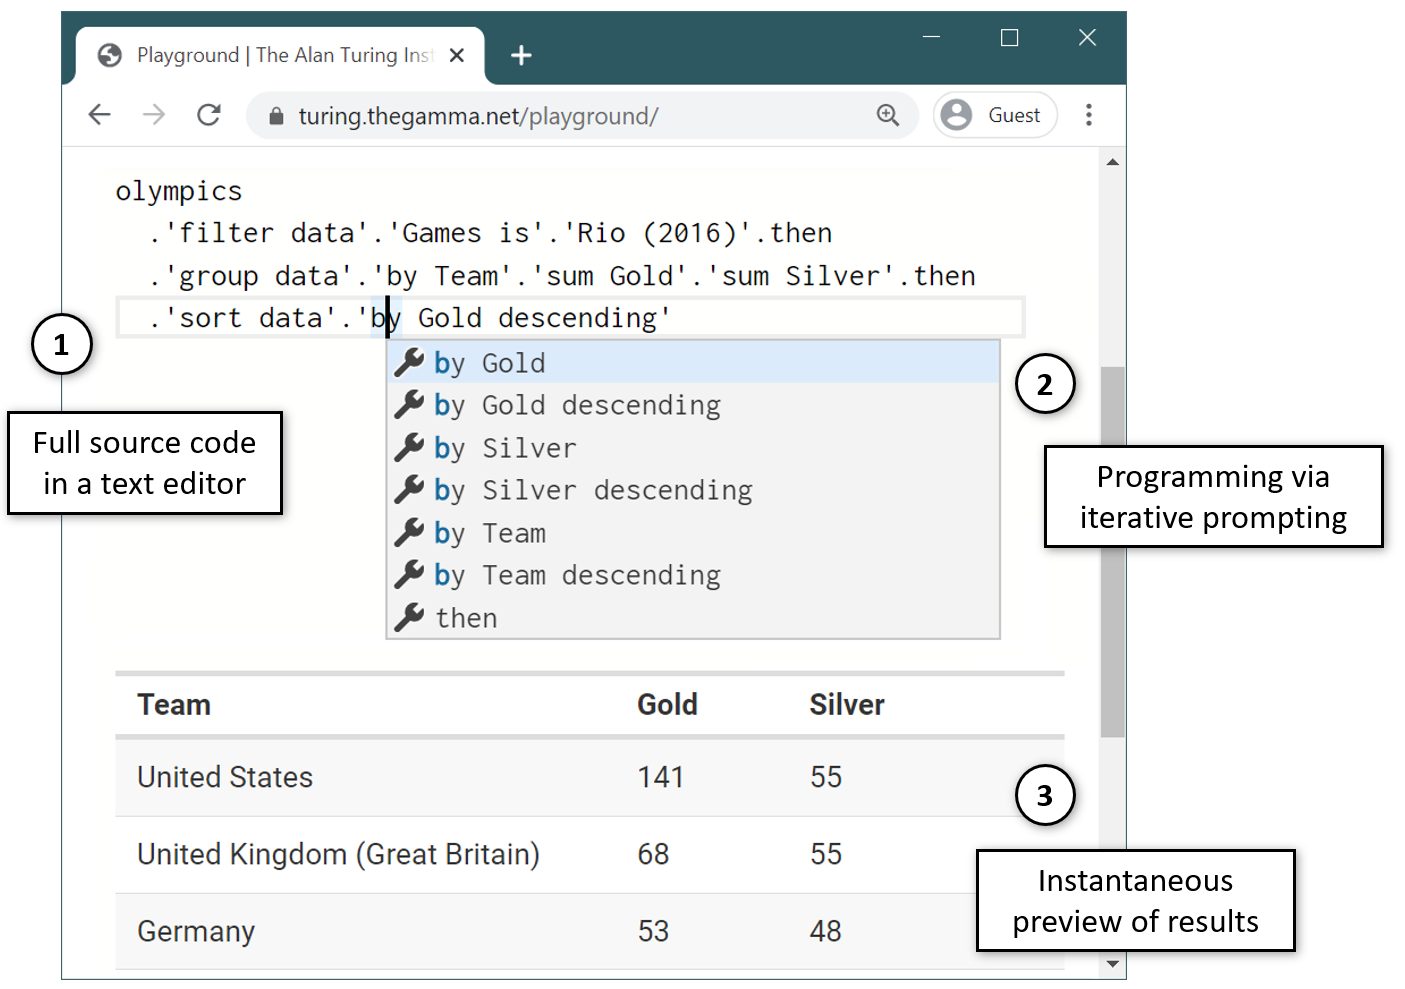
\includegraphics[width=1\columnwidth]{figures/thegamma-annot}
\caption{Teams with the greatest number of gold medals from Rio 2016
Olympics with a reproducible The Gamma script (1), an auto-complete prompt offering ways
of sorting the data (2) and instant preview (3).}
\label{fig:thegamma}
\vspace{-0.5em}
\end{figure}


\section{Introduction}
Data science has more capabilities to help us understand the world than ever before, yet at the
same time post-truth politics and increasing public distrust in statistics makes data-driven insights
increasingly less relevant in public discourse~\cite{howstatslost}. This should perhaps not be a surpirse.
Journalists can access increasing amounts of data, but producing engaging and transparent data-driven
reports that are easy to interpret is expensive and requires expert programming skills \cite{ddj}.

The design of a data exploration tool for journalists poses a unique mix of challenges. First, the
tool needs to be easy to learn for end-users working under tight deadlines. Second, it needs to
support a wide range of data sources in a way where the expertise gained when working with one data
source is relevant for other data sources. Third, the resulting data-driven insights need to be
transparent, allowing the readers to verify the claims and learn how to reproduce the work.

We present The Gamma, a text-based data exploration environment for non-experts. The Gamma
is based on a single interaction principle, which provides uniform
access to a range of data sources including data tables, graph databases and data cubes.
An anlysis created in The Gamma is a transparent script that can be followed to reproduce the
result from scratch. This allows learning from existing analyses and encourages readers
to engage with the results. Our key contributions are:

\begin{itemize}
\item We identify the design requirements for a data exploration tool for journalists
  (Section~\ref{sec:motivation}) and follow those to build a novel programming environment
  The Gamma (Section~\ref{sec:overview}).

\item We introduce \emph{iterative prompting} (Section~\ref{sec:design}),
  an interaction design principle that can be used to complete a variety of programming
  tasks in a uniform way that allows transfer of knowledge between different tasks.

\item We show how to use the iterative prompting principle for querying of distinct data
  sources including data tables, graph databases and data cubes (Section~\ref{sec:implementation}).

\item We discuss a number of case studies (Section~\ref{sec:cases}) and
  conduct a user study to evaluate the usability of The Gamma and the extent to which users can,
  (i) learn from examples and (ii)~transfer knowledge between tasks (Section~\ref{sec:study}).
\end{itemize}

The Gamma is available as open-source at \href{http://thegamma.net}{\small\bf\ttfamily thegamma.net}.

\section{Related work}

\textbf{Visual tools.}

\textbf{Programming tools.}
Notebooks

Both follow from assistant tools for software development \cite{assistants}. Our implementation,
outlined in the previous section, implements iterative prompting through a code editor mechanism
designed for code completion. Finally, the work on type providers \cite{inforich,fsdata,dotdriven},
which we extend, also utilizes code completion.


\textbf{Journalism.}
Idyll \cite{idyll}

\textbf{Type providers.}
PL work

\newpage
~
\newpage

\begin{figure}
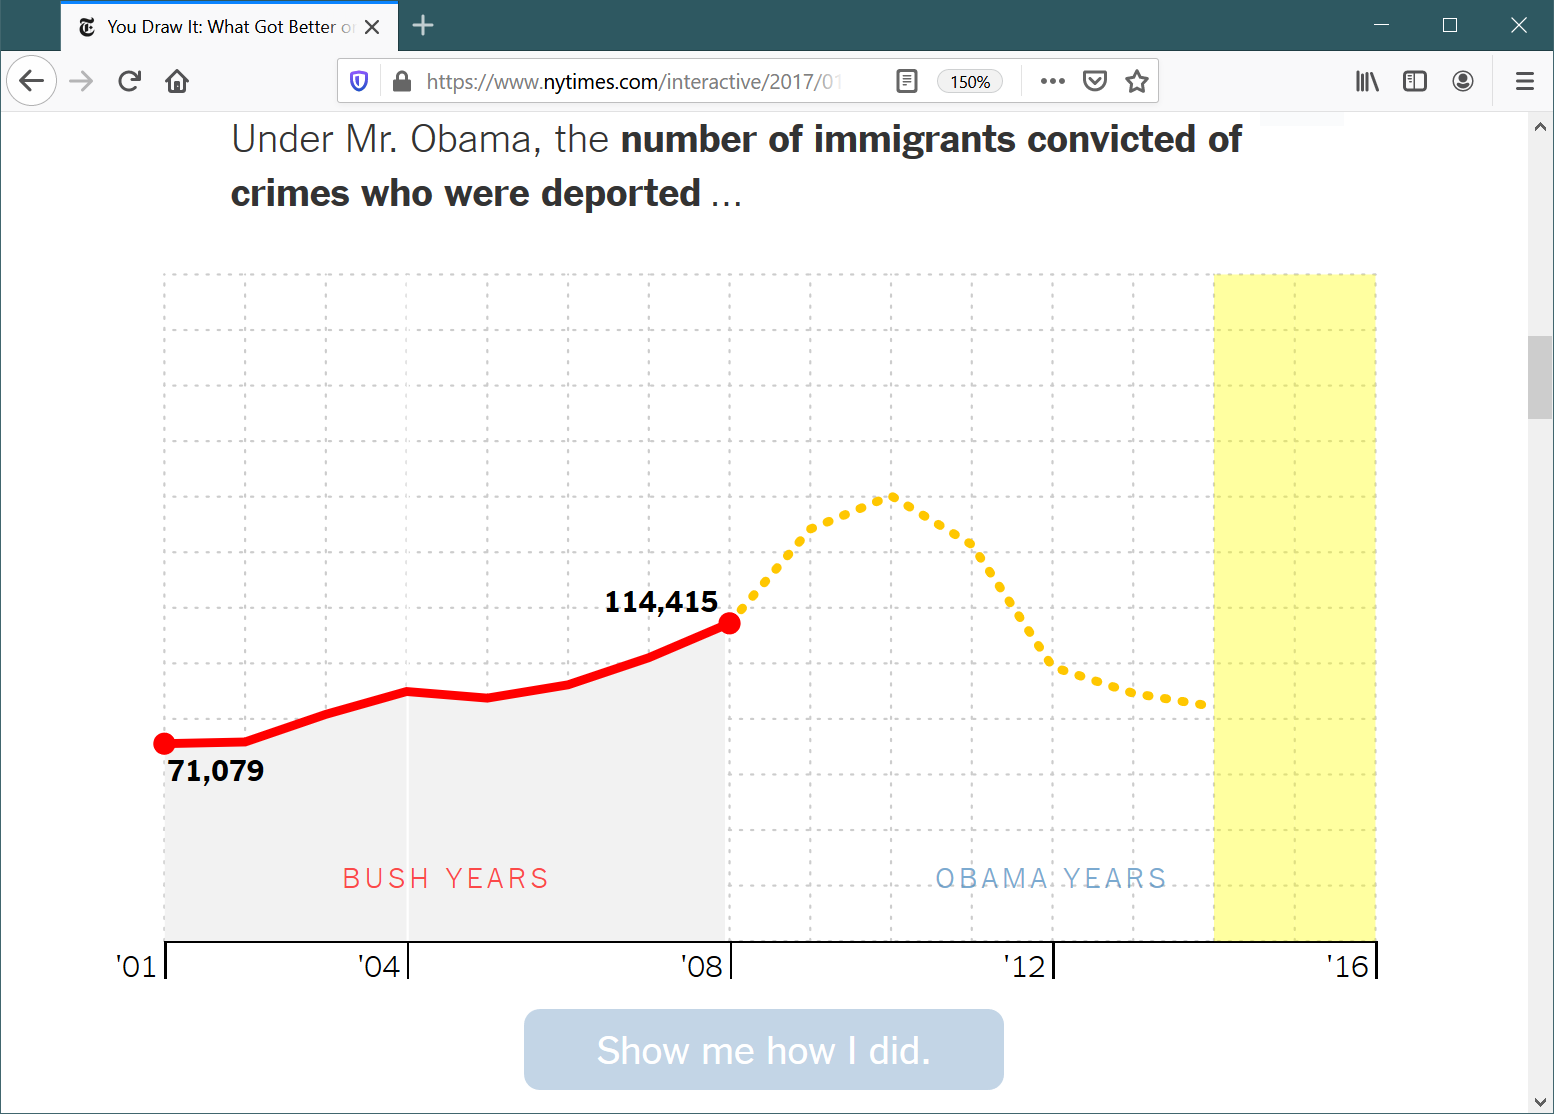
\includegraphics[width=1\columnwidth]{figures/nyt}
\caption{New York Times article on Obama's legacy \cite{youdraw}. The article asks the reader to make a guess
(engagement), but only lists ``Immigration and Customs Enforcement'' as a source of data.}
\label{fig:nyt}
\end{figure}

\section{Motivation}
\label{sec:motivation}

The Gamma aims to adapt the recent innovations in programming language research, especially the
work on type providers, into a form where it could be used in practice by journalists and other
non-expert interested in data exploration. We start with a careful consideration of our target
application domain, i.e.~data analyses produced by journalists and citizen data scientists that
are published online. We look at both practical requirements for such programming environment
and requirements arising from our focus on journalism. This analysis is based on the author's
experience of collaborating with journalists\footnote{Citations removed to preserve anonymity.},
review of literature on data journalism, e.g.~\cite{ddj,edcj17,edcj18} and more general trends in
journalism.

\subsection{Open Journalism}
Journalism continually develops and responds to the many challenges it faces \cite{future}.
Two recent challenges are relevant to our work. The first is building trust in media.
One way of establishing trust in the age of fake news is to be more transparent about editorial
decisions, process and original sources. Many journalists believe that opening up the process
shows the quality and trustworthiness of their work~\cite{transparency}.
The second challenge is reader engagement. To develop a relationship with readers, journalists are
increasingly looking for meaningful ways of engagement. This includes reader comments, involvement
of citizen journalists \cite{comments,citizen} and the development of new interactive formats
\cite{youdraw}. To address the above challenges, a tool for data exploration should satisfy the
following three requirements.

\paragraph{Trust Through Transparency}
To support trustworthiness, data analyses should be transparent. The reader should be able to
determine what is the source of analysed data and how has the data been transformed. As much as
possible, these capabilities should also be accessible to non-expert readers.

\paragraph{Reproducibility for Fact Checking}
It should be possible to re-run the analysis to verify that it produces the presented results.
However, running an opaque script is not enough. A reader should be able to recreate the analysis
by following the necessary steps from the original data source to the end result.

\paragraph{Encouraging Meaningful Engagement}
The tool should support a mechanism through which readers can engage in a meaningful discussion.
For example, it should allow modifying of parameters of a data visualization in order to show
how different choices affect the final result.

\begin{figure}
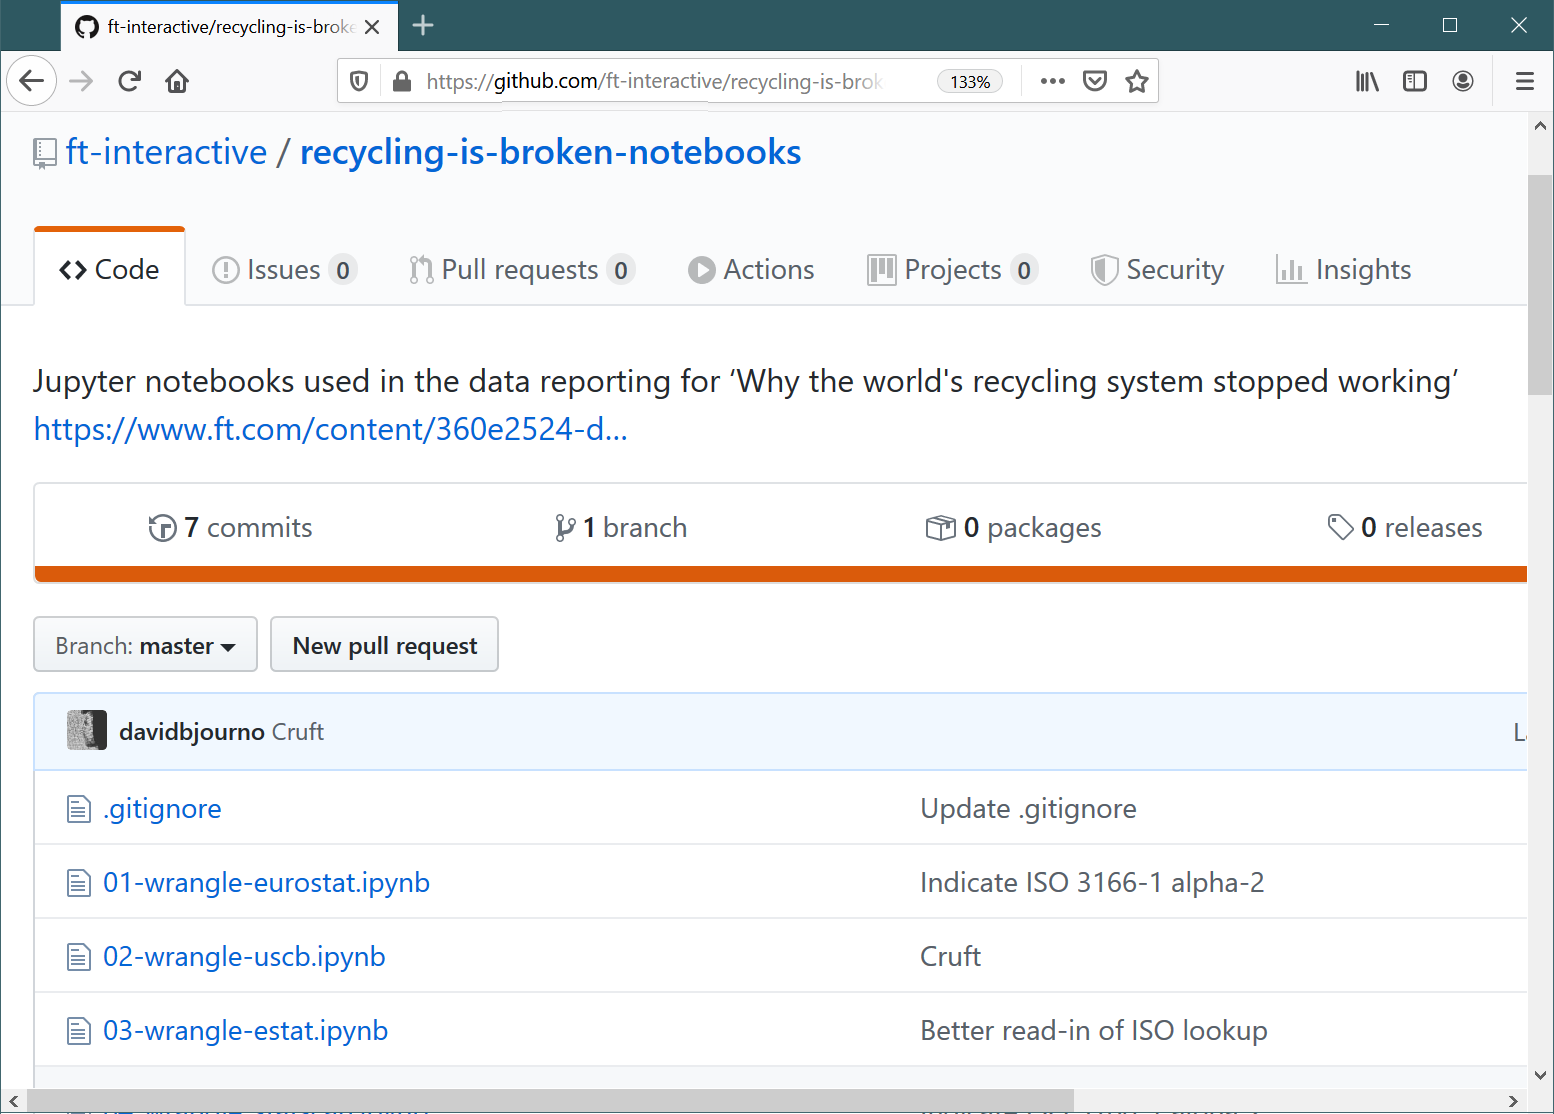
\includegraphics[width=1\columnwidth]{figures/ft}
\caption{Financial Times analysis of recyclable waste. Full source is provided as Jupyter Notebooks
on GitHub \cite{ftnotebooks}, but re-running the analysis is difficult, even for an expert.}
\label{fig:ft}
\end{figure}

\subsection{End-user Data Exploration}
Our aim is to make programmatic data exploration accessible to journalists, but we want to keep
the desirable properties of text-based programming. In particular, source code of a data
exploration should provide a full reproducible record of how the data analysis has been done.
As end-users, journalists have a number of interesting characteristics. They work under tight
deadline and data exploration is only a complementary skill. They also need to work with a wide
range of data sources, including big data tables (e.g.~Iraq War documents leak) or graph
databases (e.g.~Panama Papers). This leads to a number of practical requirements on the programming
environment.

\paragraph{Conceptual Simplicity}
We target end-users who cannot dedicate much time to learning about a tool prior
to using it. Consequently, using the tool should require understanding of only a small number
of concepts. Once the user understand a small number of concepts, they should be able to complete
basic data exploration tasks.

\paragraph{Uniformity across Data Sources}
The users should be able to navigate through large databases, query relational databases and
query graph databases through the same mechanism. Ideally, expertise gained with one data source
should also be transferable to working with another data source.

\paragraph{Learning without Experts}
Sarkar \cite{learning} reports that users learn how to use Excel either by talking to experts,
or by seeing a feature in a spreadsheet received from a colleague. In our circumstances, experts
are unlikely to be available, so the tool should support learning from examples. When looking at
a work done and published by another person, the user needs to see (and be able to understand)
how a task was completed.

\newpage
~
\newpage


\section{Overview}
\label{sec:overview}

\tg is a text-based programming environment that allows non-experts create simple data exploration
scripts using a single interaction principle -- choosing an item from an auto-complete list.
It supports a range of data sources including tabular data, graph data and data cubes.

\subsection{Querying Travel Expenses}
To introduce \tg, we walk through a simple problem that a local journalist might want to solve.
The UK government publishes travel expense claims by members of the House of Lords. A journalist
wants to find out which of the members representing the Kent county spend the most on travel.
The following shows a subset of the data:\footnote{ \url{https://www.parliament.uk/mps-lords-and-offices/members-allowances/house-of-lords/holallowances/} }

\begin{thegamma}
\textbf{Name, County, Days Attended, Days Away, Travel Costs}
Lord Adonis, London, 8, 0, 504
Baroness Afshar, Yorkshire, 2, 0, 0
Lord Alderdice, Oxfordshire, 3, 0, 114
Lord Alli, London, 5, 0, 0
Baroness Amos, London, 3, 0, 0
\end{thegamma}

After the analyst imports the CSV file (through a web interface), the environment is initialized
with code that refers to the imported variable \ikvd{expenses}. The analyst then types `.' (dot):

\begin{thegamma}
expenses.
\end{thegamma}
\vspace{-0.4em}\qquad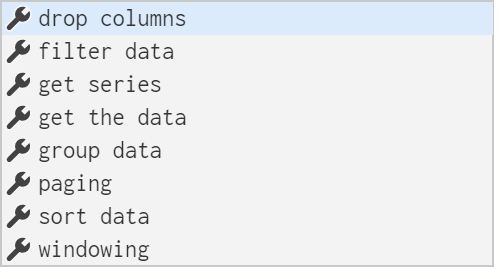
\includegraphics[width=0.5\columnwidth]{figures/lords1}

The type provider for tabular data allows analysts to construct simple queries. It first offers
a list of operations that the analyst might want to perform such as grouping, filtering and sorting.
To find members of the House of Lords from Kent, the analyst chooses \ikvd{filter data},
types `.' and then chooses \ikvd{County is} from the offered list, types `.' and starts
typing Kent:

\begin{thegamma}
expenses
  .'filter data'.'County is'.Ke
\end{thegamma}
\vspace{-0.4em}\qquad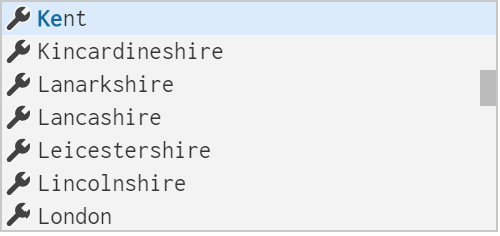
\includegraphics[width=0.5\columnwidth]{figures/lords2}

The completion list is generated from the values in the \ikvd{County} column of the dataset.
After selecting \ikvd{Kent}, the live preview is updated to only show records according to the
specified filter:

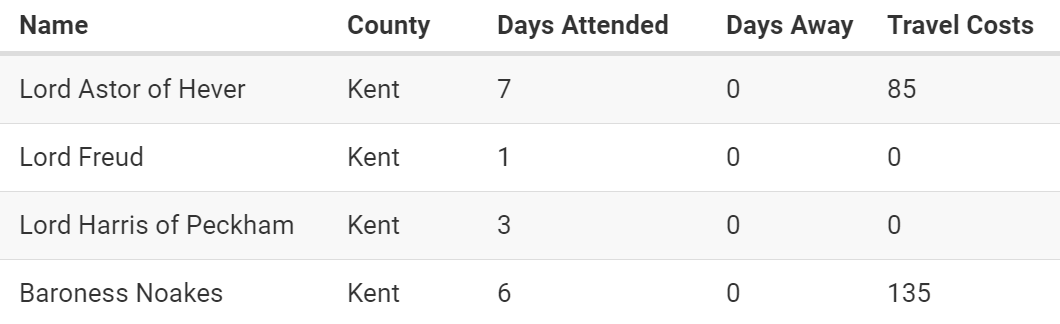
\includegraphics[width=1\columnwidth]{figures/lords3}

To finish specifying filtering conditions, the analyst chooses \ikvd{then} and is offered the
same list of querying operations as in the first step. To sort House of Lords members by their
travel costs, she now chooses \ikvd{sort data} and types `.' (dot):

\begin{thegamma}
expenses
  .'filter data'.'County is'.Kent.then
  .'sort data'.
\end{thegamma}
\qquad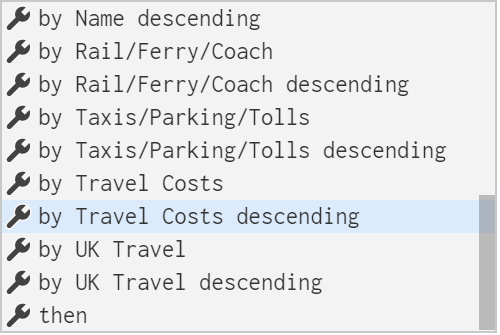
\includegraphics[width=0.5\columnwidth]{figures/lords4}

The auto-complete offers a list of columns that can be used for sorting, each with ascending
(default) and descending order option. After choosing one or more sort keys, the analyst selects
the \ikvd{then} member and is, again, offered the list of querying operations. They use
\ikvd{paging} to get top 5 records and \ikvd{get series} to obtain a data series with just
the House of Lords member name and their travel expenses.

\begin{thegamma}
expenses
  .'filter data'.'County is'.Kent.then
  .'sort data'.'by Travel Costs descending'.then
  .paging.take(5)
  .'get series'.'with key Name'.'and value Travel Costs'
\end{thegamma}

When the code evaluates to a data series with a categorical (textual) key and a numerical value,
\tg switches from displaying the result as a table to a column chart:

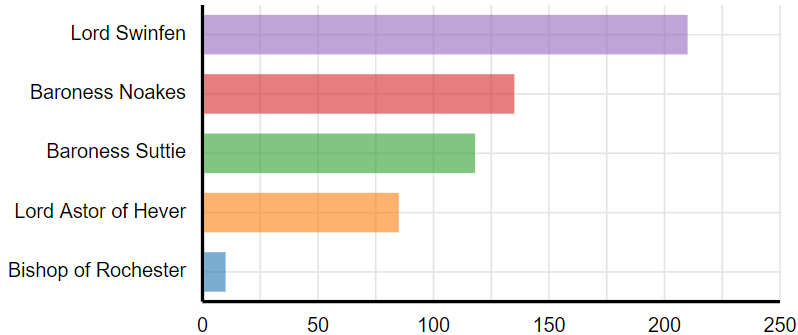
\includegraphics[width=1\columnwidth]{figures/lords5}
\vspace{-1.5em}

\subsection{Querying via Iterative Prompting}
In the example, the journalists constructs a query that filters and sorts a data table. This is
not unlike writing a query in the SQL language. However, the whole query is constructed through
a single interaction mechanism that we refer to as \emph{iterative prompting}. The user triggers
the interaction by typing `.' at the end of the query constructed so far. She is then offered a
list of available operations in the current context. This may include a choice of top-level
operations (e.g.~at the start and then again after choosing \ikvd{then}) or possible
parameters for an operation (such as possible sorting keys and directions after choosing
\ikvd{sort data}). The user then merely needs to choose one of the available options, rather than
learning the syntax and semantics of SQL in order to know what constructs can be used in the
given context.
We discuss the important aspects of The Gamma design in the next section and then discuss the
integration of specific data sources in detail, revisiting the type provider for querying
data tables.

% ==================================================================================================

\section{Design}
\label{sec:design}

We identified a number of requirements for a data exploration tool for journalists earlier.
First, using the tool should result in transparent and reproducible data analyses that can be
understood and modified by non-experts. Second, the tool should minimze the number of concepts
that the user needs to understand and, subsequently, allow them to learn through exploration
and from examples. In this section, we discuss how our design aims to satisfy those requirements.

\subsection{Lowering the Barrier to Entry}
Data exploration tasks, such as querying tables, have a certain irreducible complexity.
Regardless of the interface, the user will be exposed to concepts such as filtering,
sorting and grouping. Our design aims to lower the barrier to entry by stratifying the concepts
into first-level \emph{iterative prompting} principle and second-level \emph{domain specific
languages} for each kind of data source.
The user needs to master the iterative prompting principle in order to start working
with the system. However, using individual data sources can be mastered gradually.

\paragraph{Iterative Prompting}
Iterative prompting is an interaction principle where the user repeatedly invokes an
auto-complete prompt and makes a selection from the offered options. The principle is closely
related to both code completion and the use of command line. Iterative prompting is novel as an
overarching interaction principle for program construction.

In code completion, the auto-complete
prompt is invoked only in certain contexts, e.g.~when accessing a member of an object through a
variable defined earlier in code. It requires the user to be sufficiently familiar with the
programming language in order to get to a point where they are offered a list of members. In
contrast, our system only requires choosing the initial data source. The rest of the programming
is done via iterative prompting. The iterative nature of iterative prompting makes it similar to
using the command line or REPL (read-eval-print-loop) tools. However, those repeatedly ask the
user to type code or commands.

%https://www.nngroup.com/articles/recognition-and-recall/
We argue that iterative prompting is easier than other forms of interaction, because it
follows the \emph{recognition over recall} usability heuristic. The users are only required to
choose from an offered list of options, rather than having to recall a possible command
(to type in a command line) or a syntax in a text-based programming environment.

\paragraph{Domain Specific Languages}
The access to individual data sources in The Gamma is facilitated through a domain specific
language, which defines the primitives that are offered to the user in the auto-complete prompts
invoked through iterative prompting. The domain specific languages are embedded in The Gamma --
they define merely the available members (and specify how to evaluate a chain of members), but
they cannot define any custom syntax.

We discuss the individual domain specific languages for querying data tables, graph databases and
data cubes in a later section. The complexity of those languages differs. The previously discussed
language for querying tabular data is the most complex one. However, The Gamma makes it easy for
the user to start exploring and learning new languages, because they are all accessible via
iterative prompting.

\subsection{Building the Magic Escalator of Knowledge}
As discussed earlier, The Gamma is designed for users who work under tight deadlines and only
analyse data as their secondary task. The Gamma aims to support such users by having a low
barrier for entry and making it easy to learn independently.

\paragraph{Design for Percolation}
When analysing how Excel users learn Sarkar \cite{learning} points out that users learn new
features opportunistically when the usage of a feature is apparent in a spreadsheet. For
example, users can learn different functions to use in formulas, because those are visible in
the cell. Learning how to use a wizard for creating charts in this way is not possible because
it leaves no trace in the spreadsheet -- only the final result. Sarkar's recommendation is to
\emph{design for percolation}, i.e.~in a way where looking at the final result makes it apparent
what feature has been used and how.

\paragraph{Text-based Source Code}
In The Gamma, each step in the iterative prompting process results in an identifier that is
added to the source code. This means that a program constructed solely through iterative prompting
keeps a full trace of how it was created. Seeing the resulting source code provides the user all
information that they need to recreate the program, not just by copying it, but also by using the
iterative prompting mechanism. The Gamma represents code as text and allows the user to edit it
freely, so not all interactions leave a trace. For example, deleting the most recently selected
option and choosing a different one is not apparent from the result.

\subsection{Making Complex Things Possible}
Although the focus on The Gamma is simple data exploration and almost all the use cases we
envision can be achieved using the iterative prompting interaction principle, there remain a
few cases where more flexibility is needed. We aim to \emph{make simple things easy and
complex things possible}. The language thus supports a small number of additional constructs that
can only be used through text editing. The following example illustrates three additional
constructs:

\begin{thegamma}
\kvd{let} topTravel =
  expenses
    .'sort data'.'by Travel Costs descending'.then
    .paging.take(5).'get series'
    .'with key Name'.'and value Travel Costs'

charts.column(topTravel)
  .setTitle("House of Lords members by travel expenses")
  .setColors(["red","blue","green"])
\end{thegamma}

First, The Gamma allows operations with parameters such as \ikvd{take(3)} or \ikvd{setTitle("...")}.
This is currently needed when writing a query that skips or takes first N elements from a table.
The remaining features are not needed for basic data exploration, but allow other scenarios, such
as manual creation of charts. The \ikvd{let} construct can be used to define (immutable) variables
and The Gamma also supports lists written as \ikvd{[1,2,3]}.

% ==================================================================================================

\section{Implementation}
\label{sec:implementation}

\subsection{Language}

\subsection{Data sources}

% ==================================================================================================

\section{Use cases}
\label{sec:cases}

\newpage
~
\newpage

% ==================================================================================================

\section{User study}
\label{sec:study}

business team of a non-profit research organization, including a former journalist

\subsection{Research questions}

\paragraph{RQ1: Can end users explore data with The Gamma?}

\paragraph{RQ2: Can knowledge transfer between data sources?}

\paragraph{RQ3: Can users learn from just code samples?}

\subsection{Study design}
this is between-user user study

\subsection{Results}
it is good

\paragraph{Can end users explore data with The Gamma?}
Yes, the table shows the results.
People who spent between 10 and 25 minutes (average 18 minutes) working with The Gamma
Out of 13 people, all completed some work, 1 person completed partly and 6 were able
  to complete the task with small assistance (related to methods and syntax, as discussed below)

\begin{quote}
\emph{``This is actually pretty simple to use. You think about the logic of what you're actually asking and
    then you try to get it into the format you can. But knowing where it comes from would tell you how
    to trust it.''}
\end{quote}

we should use it as a training resource for students - would students get this?

\begin{quote}
\emph{``I don't think they'd need more than 5 minute video. This is a data
  source, this is what's in there.''}
\end{quote}

\begin{quote}
\emph{``for somebody who does not do coding or programming, this does not feel that daunting. it's not like you're giving me large screen full of code, which is reassurring" (~36)''}
\end{quote}


\paragraph{RQ2: Can knowledge transfer between data sources?}
expenditure task (#1-#5) and lords task (#9-#11) - is transfer from worldbank to expenditure and
from graph data to lords; the former transfers more directly, the latter less so (mainly because
of then and methods, which we discuss below)

\begin{quote}
  \emph{``I found it quite easy to translate what you showed us in the demo to the new dataset, i though it was quite easy to just get how that works''}
\end{quote}


\paragraph{RQ3: Can users learn from just code samples?}
in the worldbank task (#6-#9), users were given just a code sample and demo using no real
data source. They were able to complete based on just following and modifying code sample (to find other data).
(no problems they had were related to data source)

- "a video would just be this [code samples] anyway" (~19)
- "keystroke by keystroke video would be good"

\begin{quote}
  \emph{``I think providing one video of one example is good and maybe a couple of little examples of code wher people can see the kind of things you can do" (28:02)''}
\end{quote}

"more than one example of code would be useful because I'd be less confused about options"


\subsection{Further observations}

\paragraph{Making complex things possible hurts}
#11, #12, #13 all struggled with methods (they show in the completion lists)

\paragraph{Benefits and drawbacks of text}

AG - confused by indentation (Monaco inserts it automatically - duh!)
it does not work if you have it and add a new to-level thing;

BM uses copy & paste to copy thing and replace one identifier in the middle
(which would be difficult to do with non-textual representation)

people occasionally miss '.' when typing and try to use a space

\paragraph{How users understand the then keyword}

what is then: "allows us to chain together the operations"
is it special? "maybe I need it just to split over multiple lines" (experiments..) "no!"

"when you explained about the "dot then" that was a really useful thing to know. When I found that, I was like 'this is fine, this is doable'. If I knew this from the start, it would [have been easier]" (~27)

"I thought 'then' starts a new line. (...) I realised there was no 'then' after the 'paging' command. "
"It starts a new line or a new query? I assumed there would be one after 'paging' too."

\subsection{Conclusions}
(former journalist)
Do you think this is something journalists could figure out how to use?
"Yeah, I think so. There's a lot of effort going into data journalism that programming could make much quicker,
but I was always nervous about code." ... "Something like this would really simplify things."

\begin{table}
  \centering
  \begin{tabular}{l l l c l}
    \toprule
      & {\small \textit{Task}}
      & {\small \textit{Kind}} & {\small \textit{Completed}}
      & {\small \textit{Notes}} \\
    \midrule
    \small \#1 & \small expenditure & \small cube & \priority{50} & {\small Obtained one of two data series}\\
    \small \#2 & \small expenditure & \small cube & \priority{100} & {\small Explored furhter data series }\\
    \small \#3 & \small expenditure & \small cube & \priority{100}& {\small Explored further data series }\\
    \small \#4 & \small expenditure & \small cube & \priority{75}& {\small With hint to use another member }\\
    \small \#5 & \small expenditure & \small cube & \priority{100}& {\small Explored further data series }\\
    \small \#6 & \small worldbank & \small cube & \priority{75} & {\small With general syntax hint }\\
    \small \#7 & \small worldbank & \small cube & \priority{100} & {\small Completed very quickly }\\
    \small \#8 & \small worldbank & \small cube & \priority{100} & {\small Extra time to find data }\\
    \small \#9 & \small lords & \small table & \priority{75} & {\small  Struggled with composition}\\
    \small \#10 & \small lords & \small table & \priority{100} & {\small Completed very quickly }\\
    \small \#11 & \small lords & \small table & \priority{75} & {\small With a hint to avoid methods}\\
    \small \#12 & \small olympics & \small table & \priority{75}  & {\small With a hint to avoid methods}\\
    \small \#13 & \small olympics & \small table & \priority{75}  & {\small With a hint to avoid methods}\\
    \bottomrule
  \end{tabular}
  \caption{Table captions should be placed below the table. We
    recommend table lines be 1 point, 25\% black. Minimize use of
    table grid lines.}~\label{tab:table1}
\end{table}

\newpage
~
\newpage

% ==================================================================================================

\section{Discussion}

\subsection{Study limitations}
exploratory in nature so we do not make any quantitative claims about effects

not comparing against other systems

\subsection{Design principles}
How well did we do wrt design principles?

\subsection{Design issues}
future challenges and limitations of the model - such as issues when modifying code
in the middle of the call chain

\section{Conclusions}

\newpage
~
\newpage

\section{Acknowledgments}
Yo

% BALANCE COLUMNS
\balance{}

% REFERENCES FORMAT
% References must be the same font size as other body text.
\bibliographystyle{SIGCHI-Reference-Format}
\bibliography{paper}


\end{document}

%%% Local Variables:
%%% mode: latex
%%% TeX-master: t
%%% End:
